\section{Introduction}
\label{sec:intro}

Evolving graphs are used to represent a wide range of phenomena,
including the Web, social networks, communication and transportation
networks, interaction networks, metabolism pathways, and many others.
Researchers study graph evolution rate and mechanisms, impact of
specific events on further evolution, spatial and spatio-temporal
patterns, and how graph properties change over time.  \eat{We need a
  graph model that can support these types of analyses.}

The dominant logical model for evolving graphs over the past 20 years
has been a sequence of static graphs, termed {\em snapshots}.  This
model is a graph-specific adaptation of the {\em point-based temporal
  model}~\cite{Toman2009}, and it introduces a semantic ambiguity that
has been well studied in the temporal relational databases
literature~\cite{Bohlen1998}: if an entity (graph, vertex or edge)
with the same attributes exists in two consecutive snapshots, does it
represent the same fact or two different facts?  What does it mean for
an entity to change?

\begin{figure}[t!]
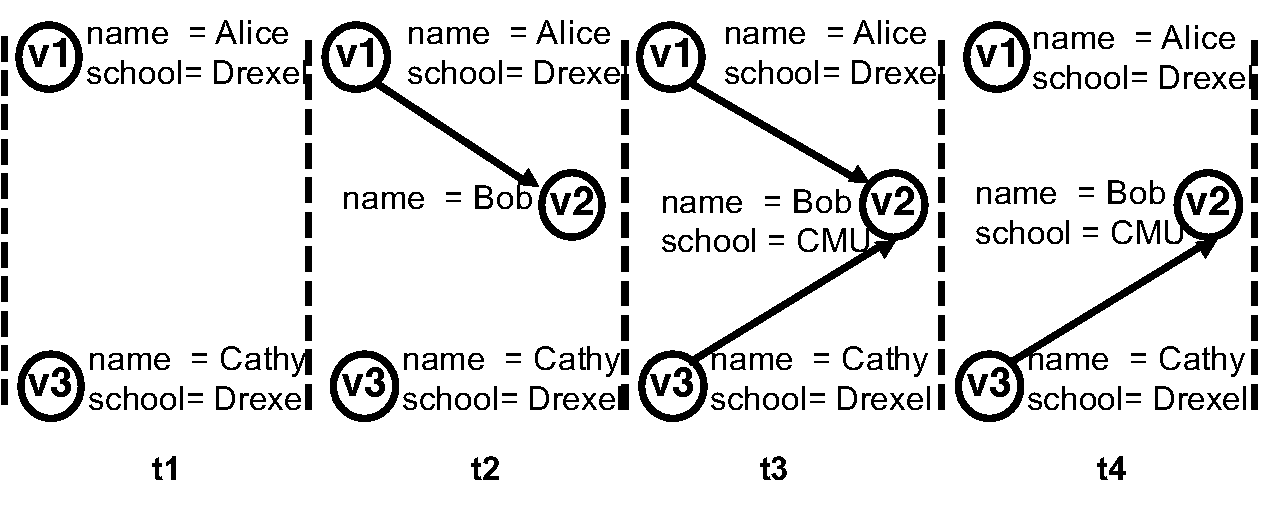
\includegraphics[width=3.4in]{figs/T1_graphs.pdf}
\vspace{-0.7cm}
\caption{A social network as a snapshot sequence.}
\vspace{-0.5cm}
\label{fig:snapshots}
\end{figure}

\begin{figure}[b!]
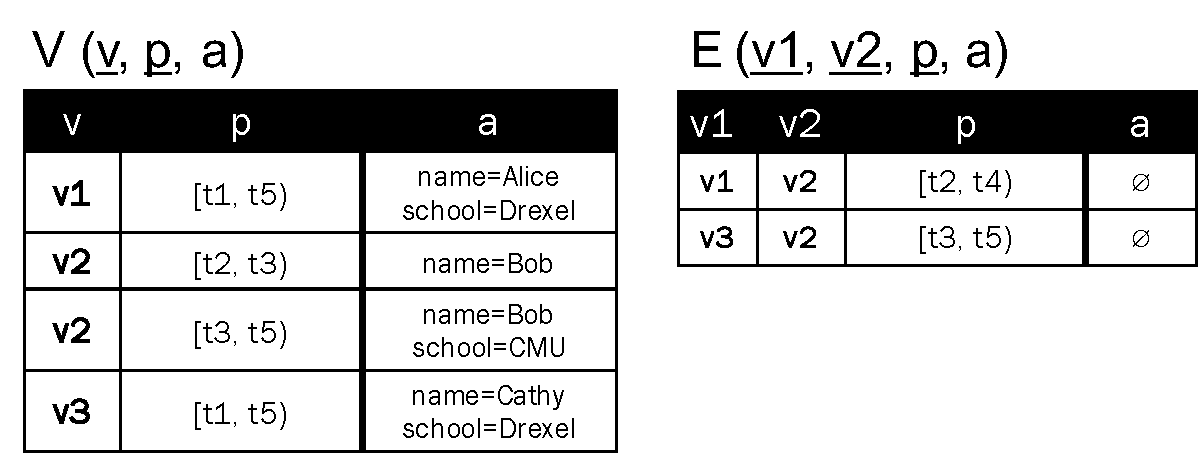
\includegraphics[width=3in]{figs/T1_relations.pdf}
\vspace{-0.2cm}
\caption{A social network as coalesced temporal relations.}
\vspace{-0.5cm}
\label{fig:coalesced}
\end{figure}

Figure~\ref{fig:snapshots} shows an example of an evolving social
network, in which vertices represent people, while edges represent
interactions between them such as likes and conversations.  In this
example, did Alice and Bob have two conversations over the time period
$[t1, t4)$ or one long one?  Did Alice undergo any changes during this
  time?  Which user was the most active in this network, as defined by
  the number of distinct interactions? What is the rate of change of
  this network?  We cannot answer these questions without additional
  information in a point-based model.  Suppose that Alice held a
  temporary position at Drexel at time $t1$ and transferred to a
  permanent one at time $t2$.  This information cannot be represented
  in the point-based model.  Suppose that Alice and Bob had two short
  interactions, while Cathy and Bob had one longer one.  The
  point-based model cannot distinguish between these two cases.

This kind of semantic ambiguity affects several graph operations, most
notably aggregation and retrieval of change history, and, as a result,
local (confined to specific entity or subset of entities) and global
(whole-graph) temporal queries that are useful for evolving graph
analysis.

In a point-based model~\cite{Toman2009} each entity is time-stamped
with its validity time.  For practical reasons, intervals are often
used as syntactic abbreviations for sets of points.  To use intervals
in a time-stamped model, we coalesce, i.e., merge value-equivalent
tuples over overlapping and adjacent time points~\cite{Bohlen09}.
Figure~\ref{fig:coalesced} represents the network of
Figure~\ref{fig:snapshots} as a pair of coalesced temporal relations
--- \insql{V} for vertices and \insql{E} for edges.  Vertex and edge
attributes are represented as sets of key-value pairs based on the
property graph model~\cite{Angles2008}.

Importantly, the use of intervals to represent a sequence of
value-equivalent time-adjacent snapshots is not semantically
equivalent to a model with {\em sequenced semantics}, where entities
are time-stamped with intervals that have meaning.\eat{ Note that
  Alice shows no changes during the whole time interval, with a single
  tuple over $[t1, t4)$.  Similarly, two interactions between Alice
    and Bob are coalesced into one.} A work-around to avoid coalescing
  tuples that represent different facts is to add attributes to
  entities, in order to distinguish between changes and non-changes.
  For example, we can add position title to the vertex Alice to state
  that Alice changed jobs at time $t2$, and add a conversation id to
  each edge to designate distinct conversations.  Unfortunately, this
  solution is ad-hoc rather than general and does not hold up over
  time, as discussed in~\cite{Bohlen1998}.

\eat{With sequenced semantics Alice is represented with two tuples,
  one for each interval corresponding to a separate position.}

\eat{Besides the semantic ambiguity problem, many queries cannot be
  formulated over a point-based graph model.  In particular, any query
  with a temporal predicate, e.g., compute a subgraph containing only
  vertices that persist for at least a year, cannot be formulated over
  the snapshot sequence because semantically the query is computed
  independently in each snapshot.}

We contend that a snapshot sequence model of evolving graphs is
insufficient for representation of a wide range of networks\eat{.  We
  gave an example above, but in general any network where consecutive
  tuples may represent different facts while being value-equivalent is
  affected. To address this issue, we} and propose instead to use the
interval model with sequenced semantics. Facts in our model correspond
to graph vertices and edges (as in Figure~\ref{fig:coalesced}), rather
than to graph snapshots in their entirety (as in
Figure~\ref{fig:snapshots}).  This representational choice is
orthogonal to the issue of point-based vs. sequenced semantics, but
has an important advantage.  Many evolving graph queries include
temporal predicates over vertices or edges, e.g., compute a subgraph
containing only vertices that persist for at least a year.  Such
queries cannot be evaluated directly over a sequence of snapshots.

\eat{ Interaction networks, such as message exchange graphs,
  epidemic transmission networks, network topologies, and any graphs
  with events as edges are cases where this issue is more likely to
  appear (the graphic example above is of an interaction network).}
\eat{Besides the semantic ambiguity problem, many queries cannot be
  formulated over a point-based graph model.  In particular, any query
  with a temporal predicate, e.g., compute a subgraph containing only
  vertices that persist for at least a year, cannot be formulated over
  the snapshot sequence because semantically the query is computed
  independently in each snapshot.}
%

In Section~\ref{sec:related} we briefly survey existing models and
summarize relevant work in temporal databases.  We then propose a new
model in Section~\ref{sec:model}.  In Section~\ref{sec:consider} we
discuss the challenges of efficient computation under sequenced
semantics in a distributed environment.  We conclude with future
research directions in Section~\ref{sec:conc}.



